\documentclass[a4paper]{report}
\usepackage[utf8]{inputenc}
\usepackage[portuguese]{babel}
\usepackage{hyperref}
\usepackage{a4wide}
\hypersetup{pdftitle={MDIO - Trabalho 2},
pdfauthor={João Teixeira, José Ferreira, Miguel Solino},
colorlinks=true,
urlcolor=blue,
linkcolor=black}
\usepackage{subcaption}
\usepackage[cache=false]{minted}
\usepackage{listings}
\usepackage{booktabs}
\usepackage{multirow}
\usepackage{appendix}
\usepackage{tikz}
\usepackage{authblk}
\usepackage{bashful}
\usepackage{verbatim}
\usepackage{amsmath}
\usepackage{tikz}
\usepackage{tikz,fullpage}
\usetikzlibrary{arrows,%
                petri,%
                topaths}%
\usepackage{tkz-berge}
\usetikzlibrary{positioning,automata,decorations.markings}
\AfterEndEnvironment{figure}{\noindent\ignorespaces}

\begin{document}

\title{MDIO - Trabalho 2\\ 
\large Grupo Nº 3}
\author{João Teixeira (A85504) \and José Ferreira (A83683) \and Miguel Solino (A86435)}
\date{\today}

\begin{center}
    \begin{minipage}{0.75\linewidth}
        \centering
        
\includegraphics[width=0.4\textwidth]{images/eng.jpeg}\par\vspace{1cm}
        \vspace{1.5cm}
        \href{https://www.uminho.pt/PT}
        {\color{black}{\scshape\LARGE Universidade do Minho}} \par
        \vspace{1cm}
        \href{https://www.di.uminho.pt/}
        {\color{black}{\scshape\Large Departamento de Informática}} \par
        \vspace{1.5cm}
        \maketitle
    \end{minipage}
\end{center}

\tableofcontents

\pagebreak

\chapter{Introdução}
Um dos problemas \textit{NP-Completo} mais conhecido é o \textit{Travelling
Salesman Problem}. \\
Neste problema, um vendedor tem um conjunto de cidades que pretende visitar. As
estradas entre essas cidades e e a distancia destas também são conhecidas. O
objetivo deste problema é calcular o caminho mais curto que visite todas as
cidades.\\
Quando transferido para um grafo orientado, este problema resume-se
encontrar o caminho mais curto que visite todos os nodos do grafo.\\
Um problema derivado do \textit{Travelling Salesman Problem} é o \textit{Chinese
Postman Problem}.\\
Neste, um carteiro pretende entregar todas as cartas que tem, e para isso tem de
passar em todas as ruas pelo menos uma vez. Com o objetivo de percorrer a menor
distância possível.\\
Quando transferido para um problema de grafos, a única diferença entre este
problema e o problema do caixeiro viajante é que se pretende obter o caminho
mais curto que visite todos os arcos de um grafo orientado. \\
O objetivo deste projeto é resolver este problema utilizando \textit{RELAX4} e 

\chapter{Parte I}
\section{Problema}
Observando os números de inscrição dos membros do grupo, constatamos
que o maior pertencia ao aluno Miguel Solino (86435).
Fazendo \textit{pattern matching} para o padrão ABCDE e seguindo as
regras definidas no enunciado, concluímos que a orientação das ruas é:

\begin{enumerate}
    \item A é igual a 8;
    \item B é igual a 6, logo é par, e por isso aponta para baixo;
    \item C é igual a 4, logo é par, e por isso aponta para a direita;
    \item D é igual a 3, logo é ímpar, e por isso aponta para cima;
    \item E é igual a 5, logo é ímpar, e por isso aponta para a 
        esquerda;
\end{enumerate}
Assim, conclui-se que o problema a resolver é representado pela
seguinte imagem:

\begin{figure}[H]
    \begin{center}
        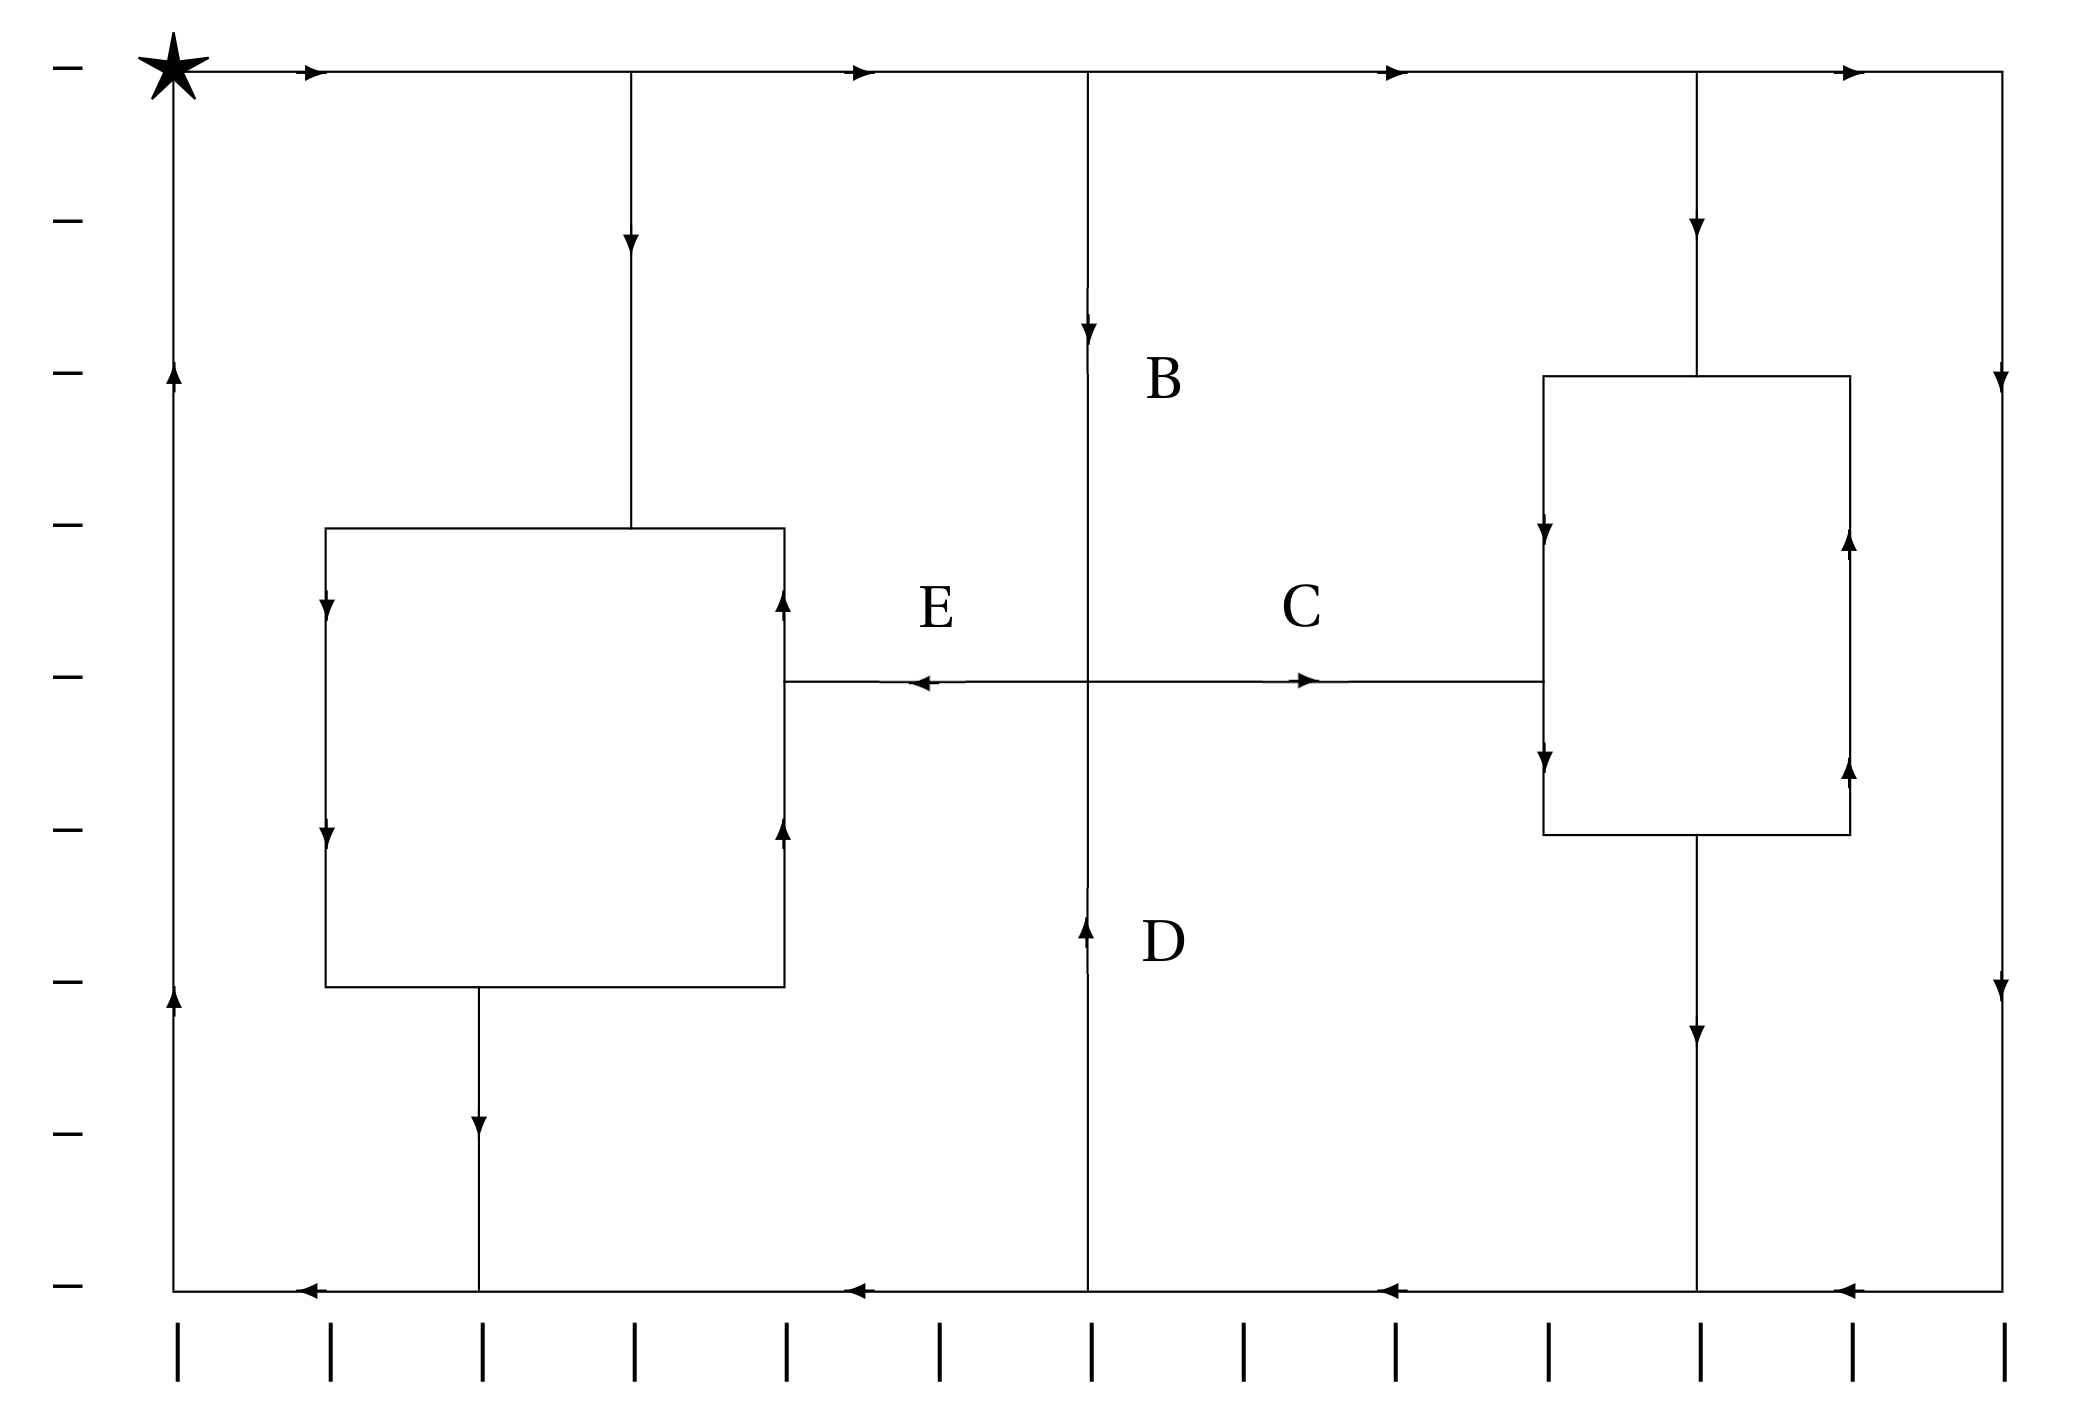
\includegraphics[width=0.9\textwidth]{images/desafio.png}\par
        \caption{representação do problema}
        \label{fig:problem}
    \end{center}
\end{figure}
Após obter esta imagem decidimos nomear cada vértice do problema com
uma letra maiúscula. Assim, o aspeto do desafio final utilizada é:

\begin{figure}[H]
    \begin{center}
        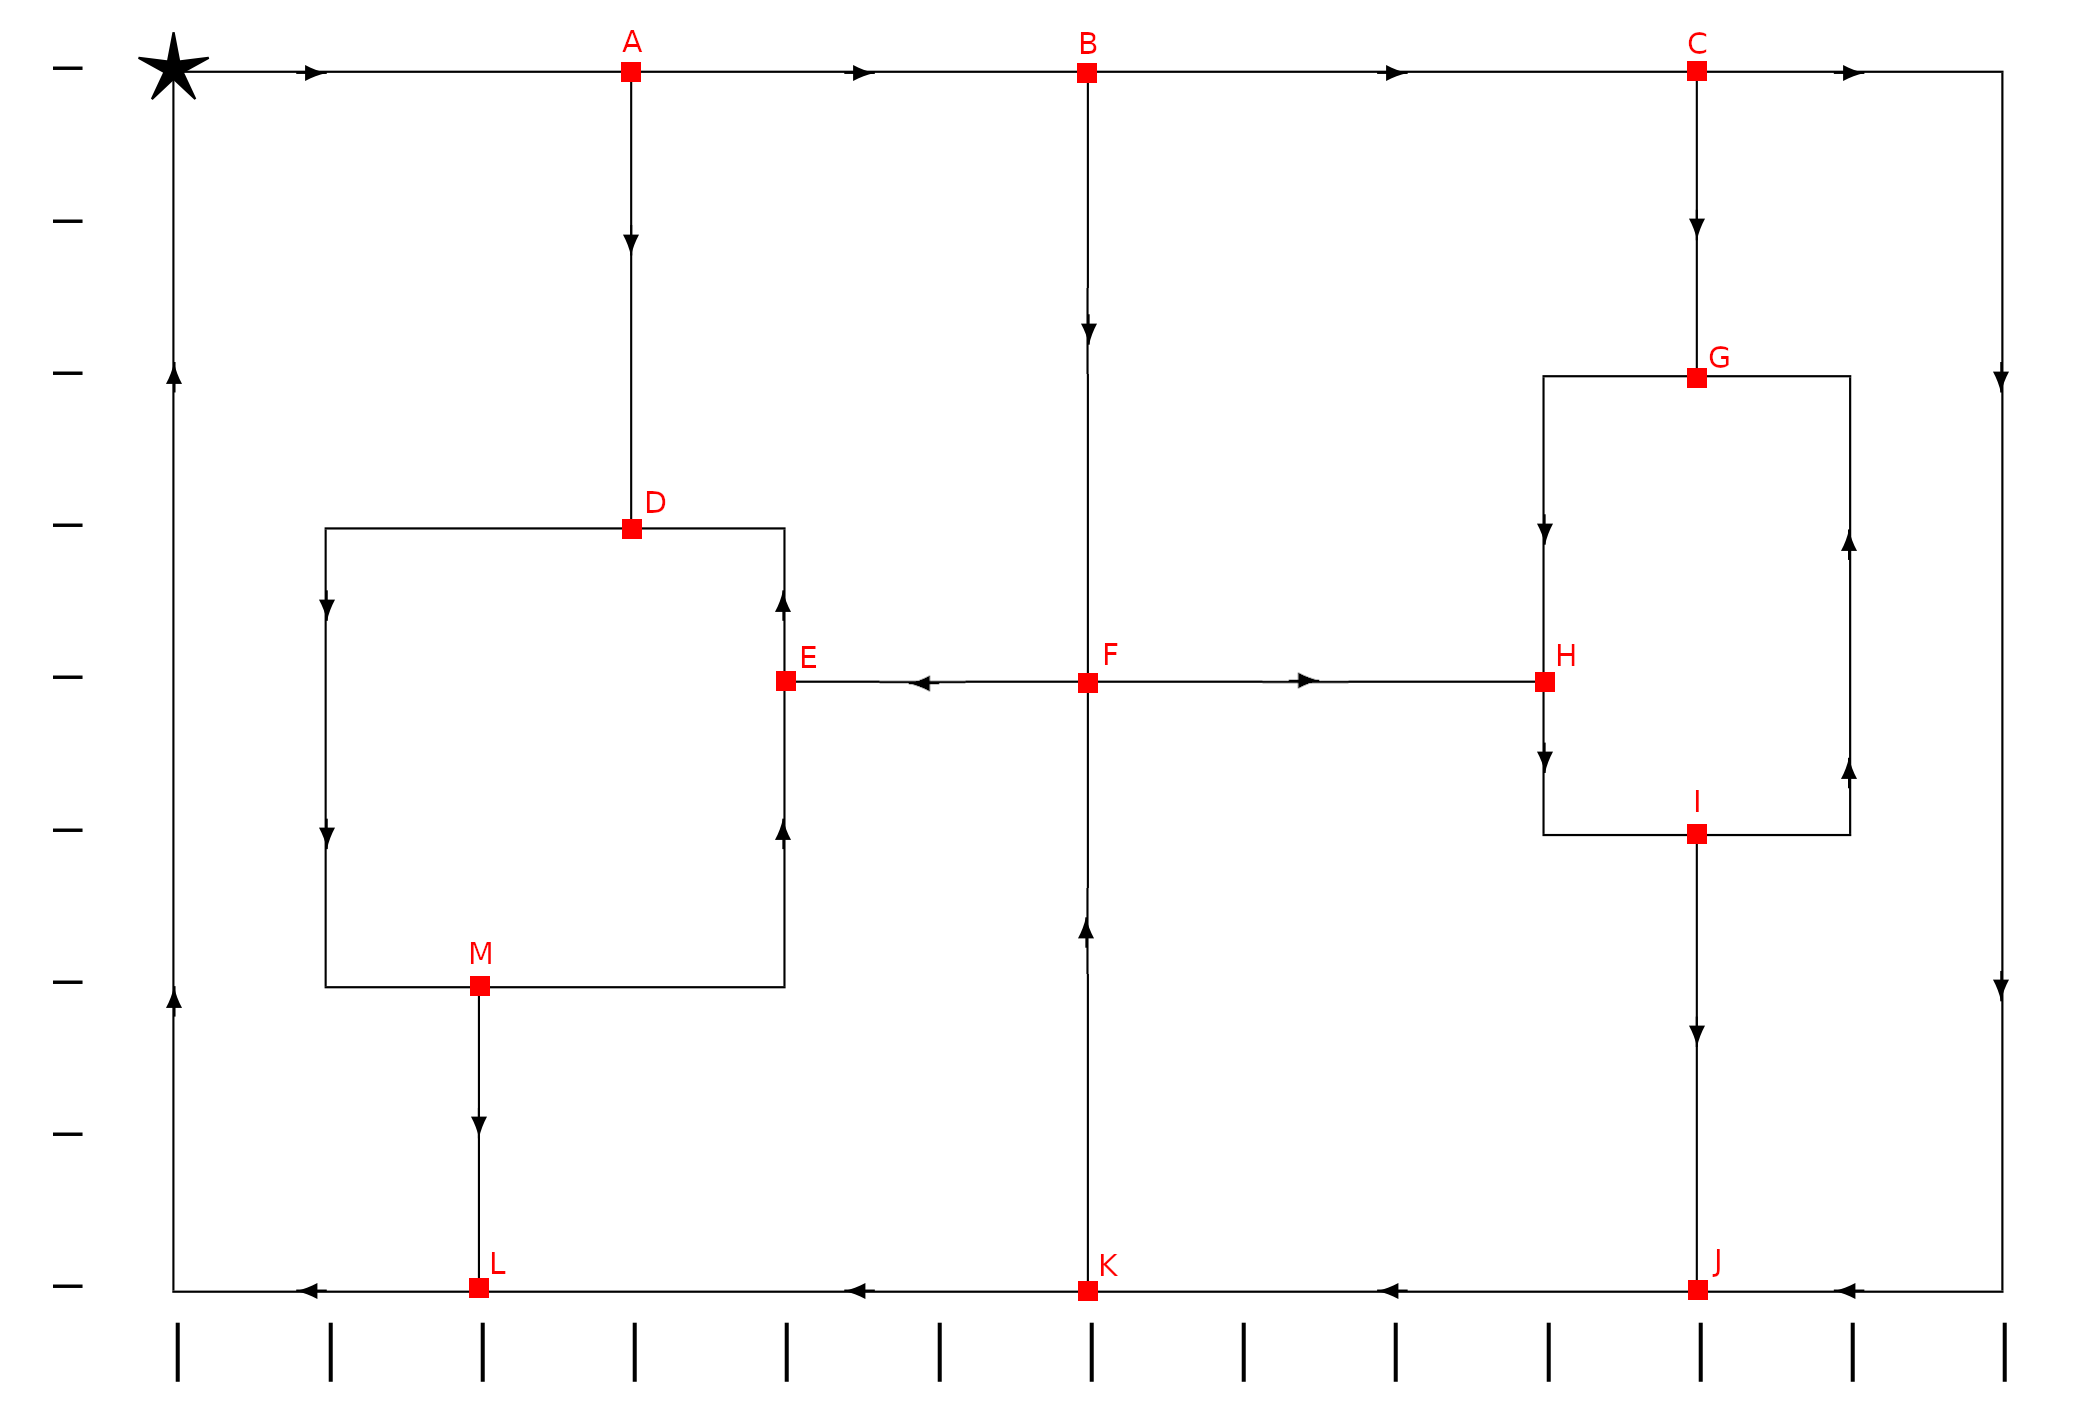
\includegraphics[width=0.9\textwidth]{images/desafioLetras.png}\par
        \caption{vértices nomeados}
        \label{fig:named}
    \end{center}
\end{figure}

\pagebreak
\section{Formulação do Problema}
Para esta primeira parte, o problema apresentado deve ser formulado como um
problema de transporte numa rede geral \textit{G=(V, A)}.

\subsection{Arestas}
A variável de decisão \textit{xij} representa o número de vezes que o arco (i,
j) foi percorrido.\\
Visto que o objetivo deste problema é que cada arco seja atravessado pelo menos
uma vez, é necessária a existencia de um bloco de condições que indiquem que
\textit{xij >= 1}.\\
No entanto, o \textit{software} de resolução de problemas em rede normalmente
apenas suporta arcos com um limite superior. Assim, aplica-se a mudança de
variável \textit{yij = xij - lij} em que \textit{lij} é o limite inferior de
fluxo no arco (i, j). Visto que o objetivo é visitar todas os arcos do grafo
pelo menos uma vez esta é igual a 1.\\
Aplicando esta mudança de variável à condição acima descrita obtemos que
\textit{xij >= 1} é equivalente a \textit{yij >= 0}.

\subsection{Nodos}
Para cada nodo no mapa, a soma de todas as vezes que se entra neste
tem de ser igual à soma de todas as vezes que se sai.\\
Assim, por exemplo, para o nodo A, o número de vezes que o arco \textit{xla} é
percorrido tem de ser igual ao número de vezes que os arcos \textit{xad} e
\textit{xab} são percorridos.
Por exemplo, de forma a criar uma restrição para o nodo A, esta pode ser
formulada como:\\
\begin{multline}
- xla + xad + xab = 0 \\
\end{multline}
Aplicando a mudança de variável:
\begin{multline}
- (yla + 1) + (yad +1) + (yab +1) = 0 \\
\end{multline}
que pode ser simplificado para:
\begin{multline}
- yla + yad + yab = -1\\
\end{multline}

\pagebreak
\section{Modelo de Programação Linear alterado}
\verbatiminput{solution.PT1.lp}

\pagebreak
\section{Rede do Problema de Transporte}

\begin{figure}[H]
    \begin{center}
        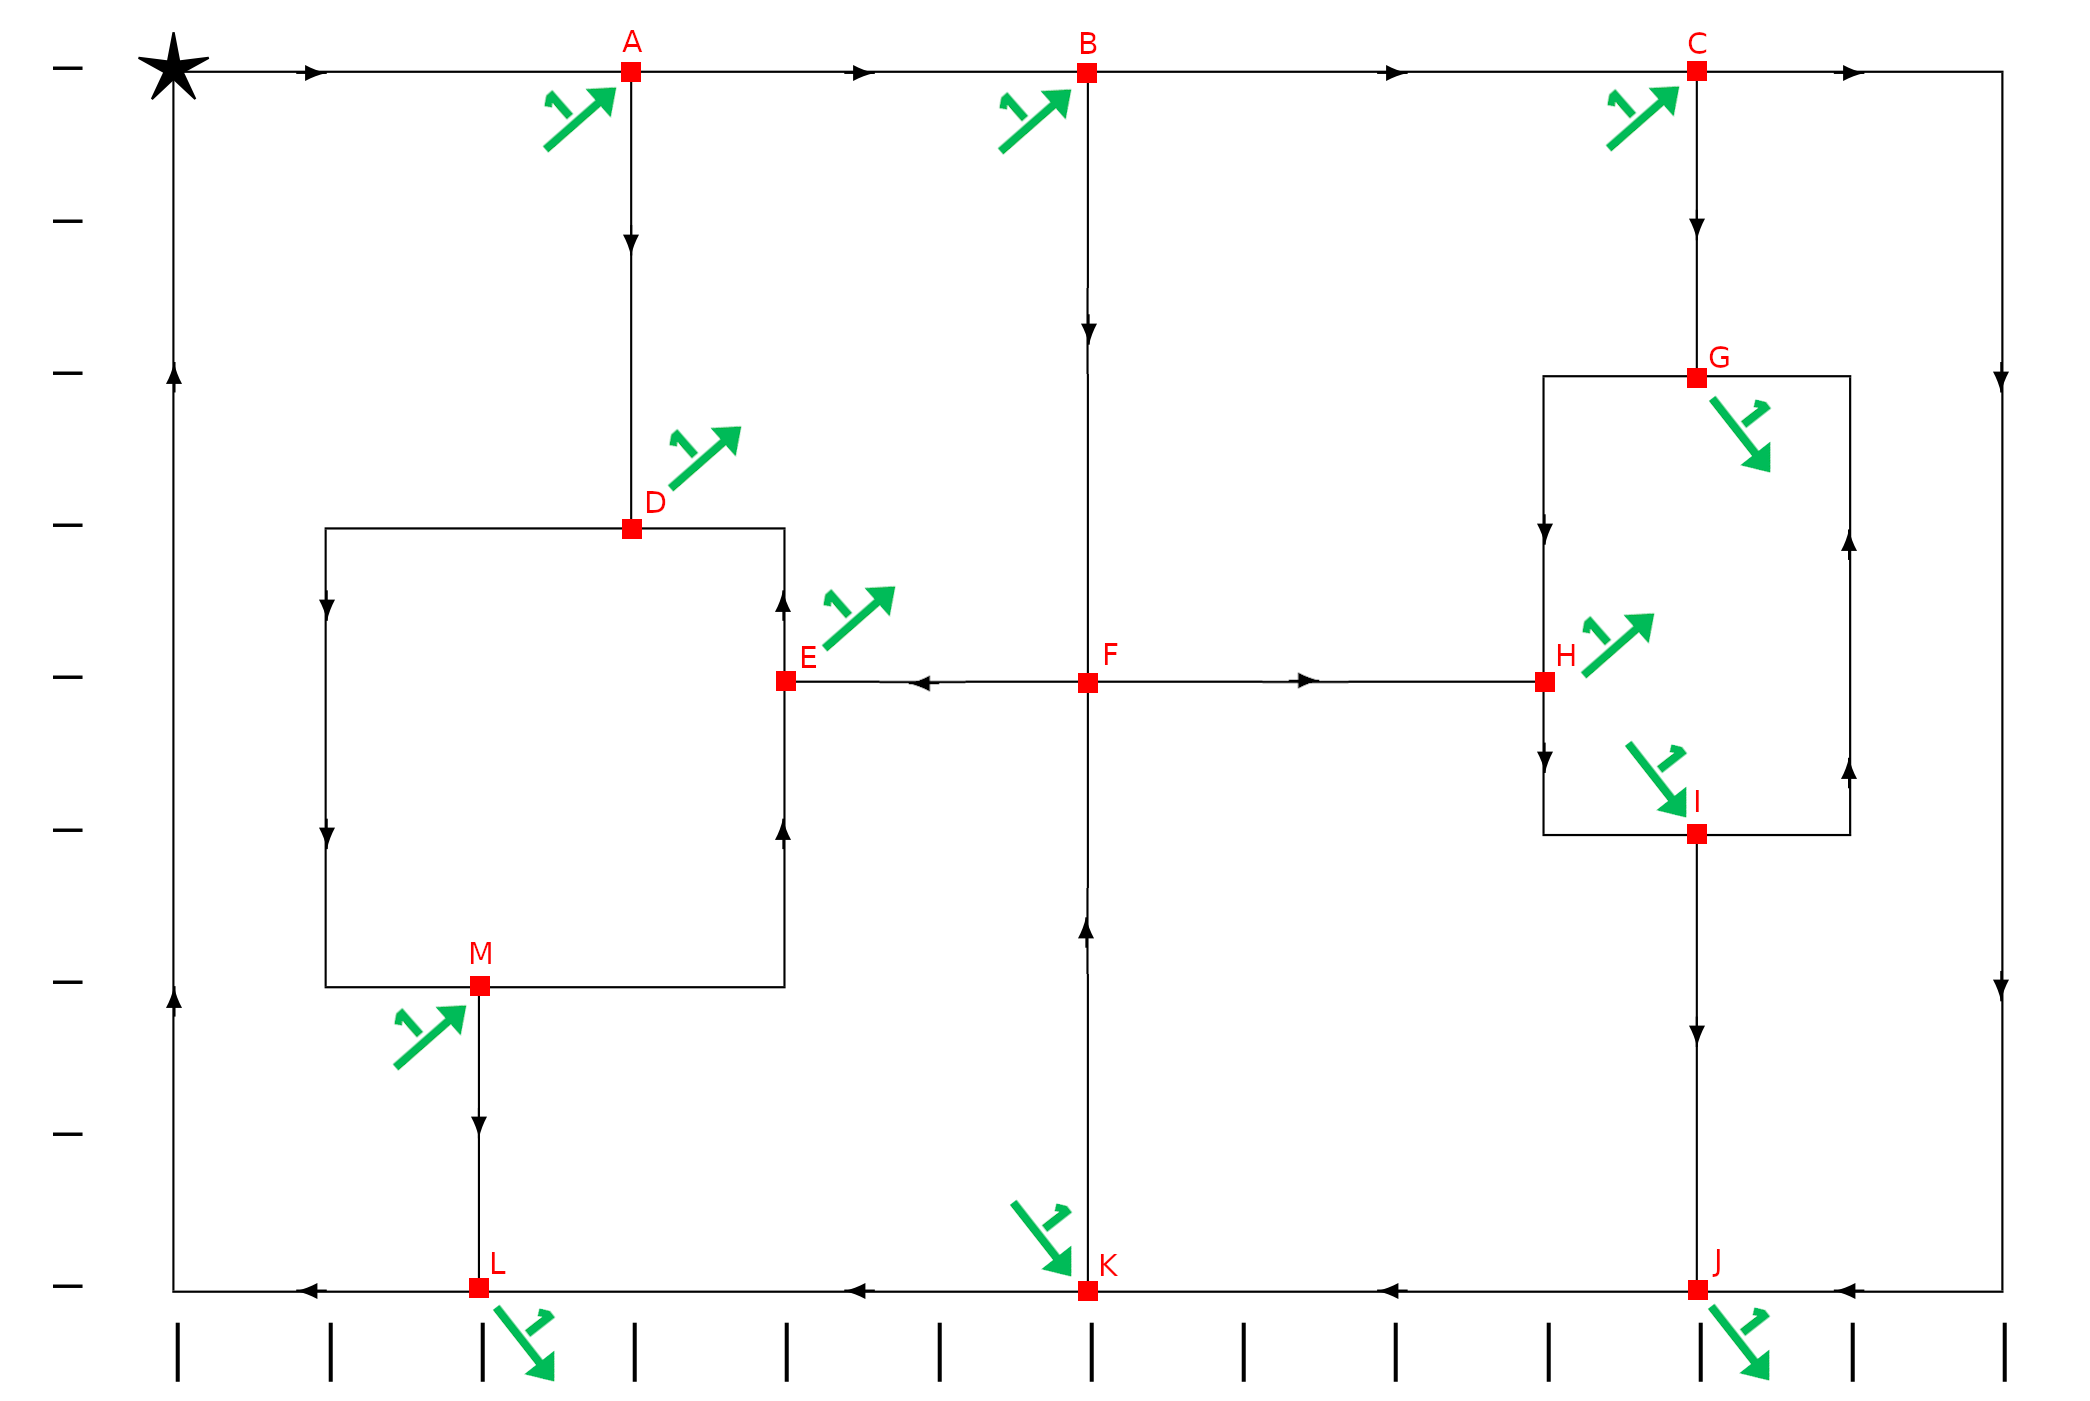
\includegraphics[width=0.9\textwidth]{images/redeTransporte.png}\par
        \caption{rede do problema de transporte}
        \label{fig:redeTransporte}
    \end{center}
\end{figure}
De forma a que o input gerado para o \textit{RELAX4} seja válido é necessário
converter o nome dos nodos para números. Assim, o método utilizado é atribuir
como número a cada nodo o valor da posição da letra no alfabeto.


\pagebreak
\section{Texto de Input}
\label{input}
\verbatiminput{RELAX4.PT1.INP}

\pagebreak
\section{Texto de Output}
\label{output}
\verbatiminput{RELAX4.PT1.OUT}

\pagebreak
\section{Interpretação do resultado}
\label{solution}
O valor obtido com o recurso ao \textit{relax4} é 87 (primeira linha do texto de
output). Uma vez que foi realizada uma mudança de variável, todos os arcos foram
visitadas n+1 vez do que a que é indicada na solução. Logo, para obter o custo
real do percurso obtido, é necessário somar ao valor obtido a soma de todos os
custos dos arcos do grafo.\\
Assim, o custo do percurso obtido é igual a 87 + 85, que é igual a 172.\\
Visto que a solução ótima é um circuito fechado, independentemente do ponto
que se considere como o ponto inicial, este será sempre o mesmo. \\
Assim, de forma a facilitar a interpretação dos resultados consideramos como
ponto inicial o ponto A. Esta decisão em nada altera o problema.\\
A fim de facilitar a visualização dos resultados obtidos decidimos criar uma
imagem \ref{fig:visited} que indica para cada arco o número de vezes que este
foi atravessado omitindo aqueles que nunca são atravessados.

\begin{figure}[H]
    \begin{center}
        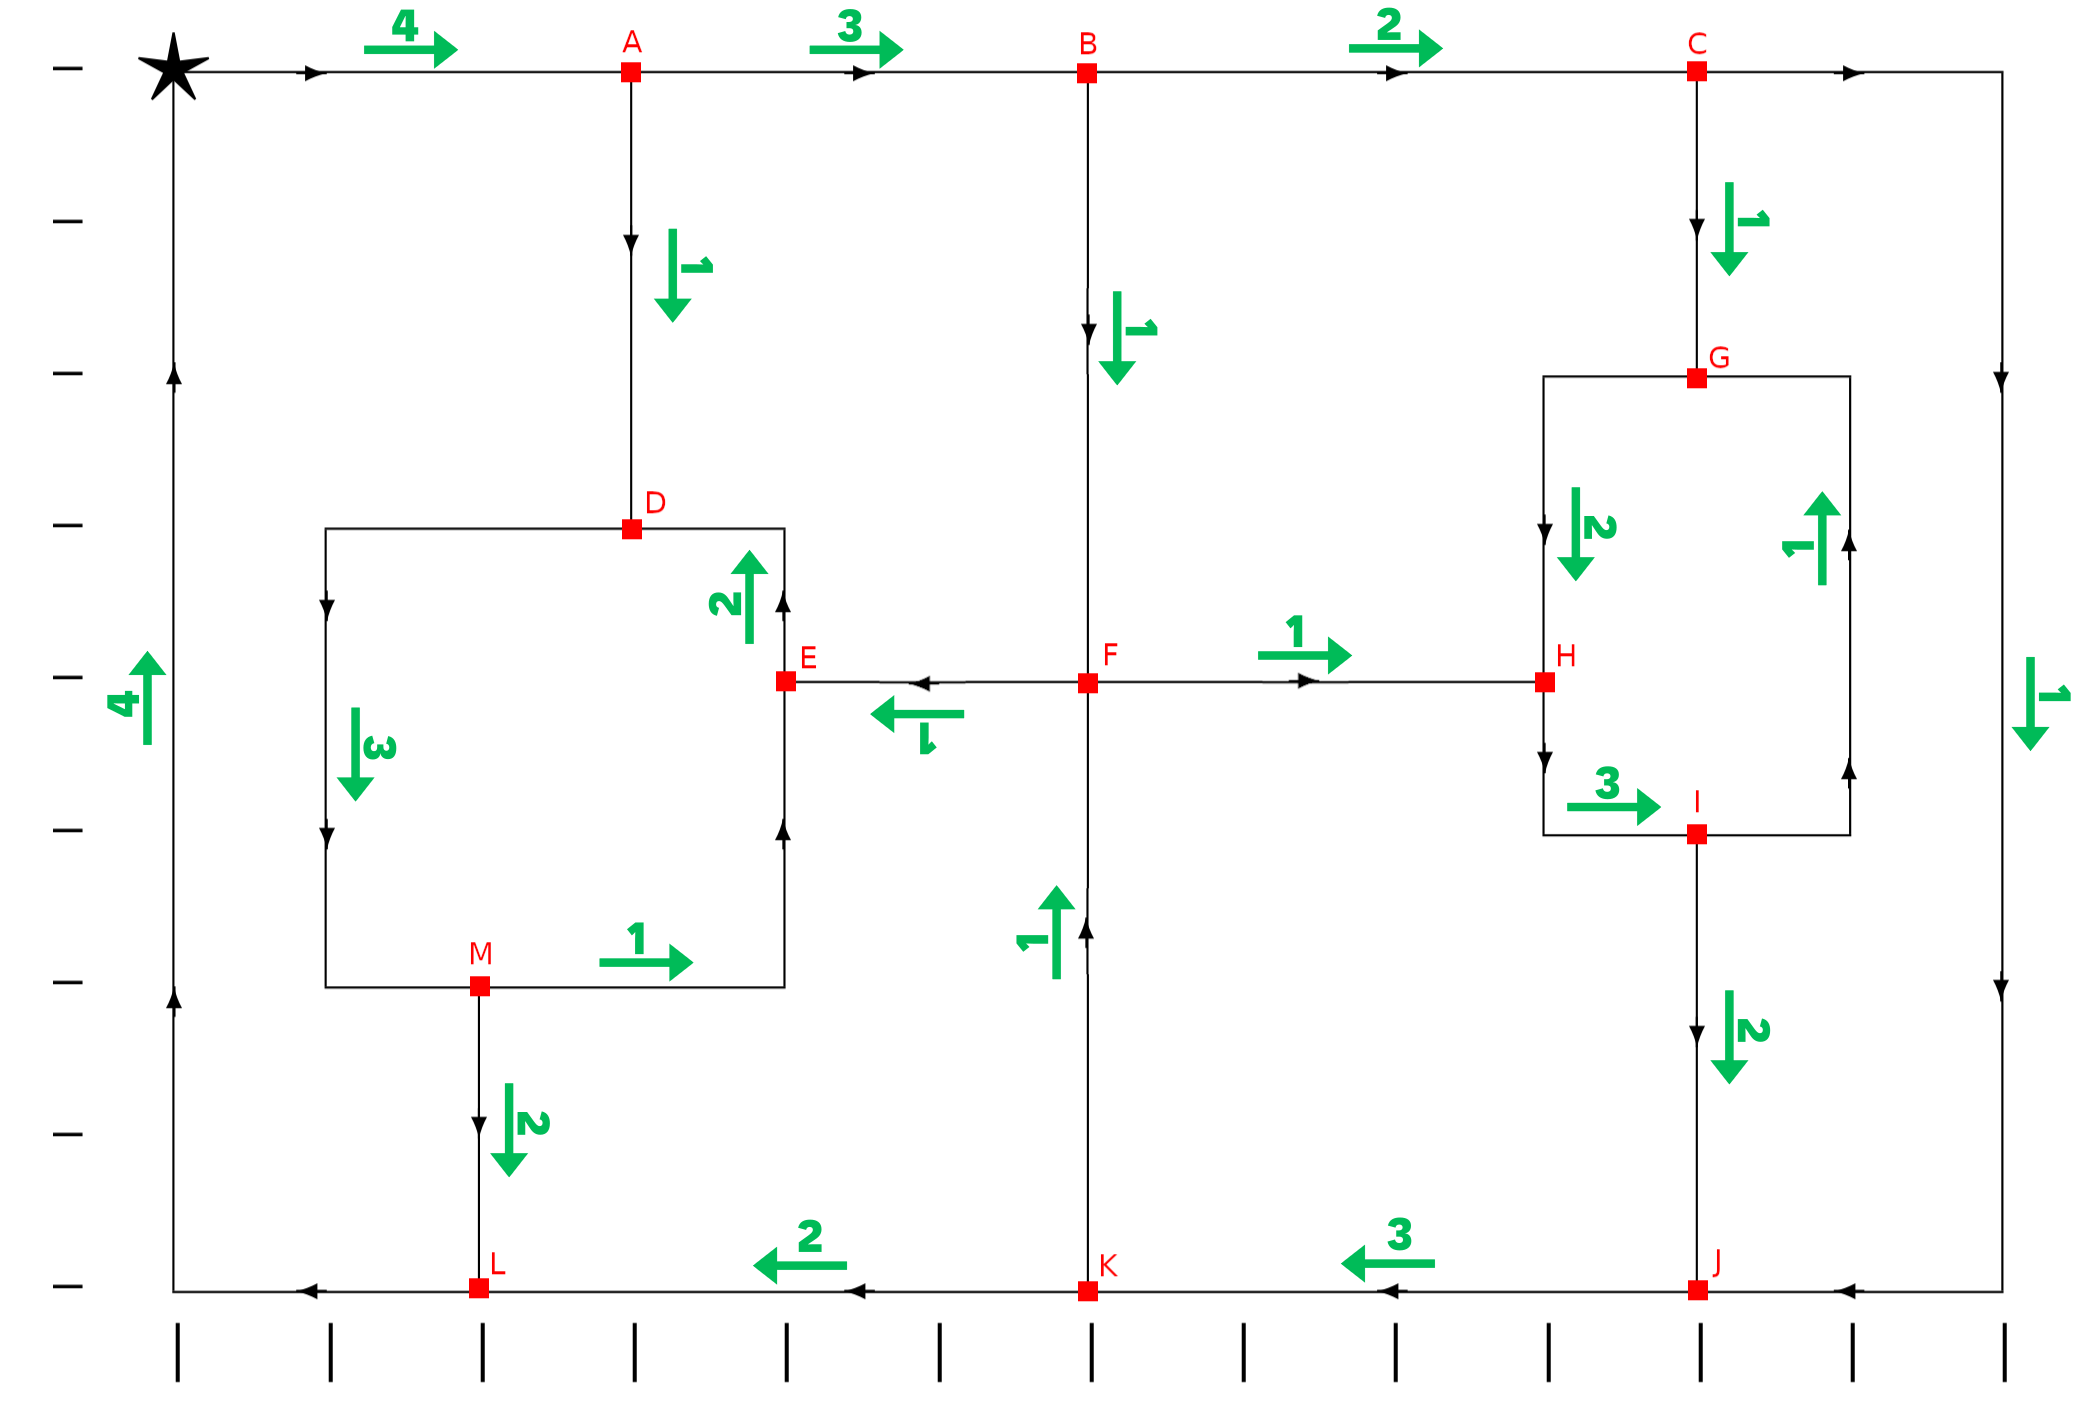
\includegraphics[width=0.8\textwidth]{images/desafioVisited.png}\par
        \caption{representação da solução}
        \label{fig:visited}
    \end{center}
\end{figure}
Analisando esta imagem, conseguimos obter o conjunto ótimo de caminhos de
reposicionamento entre os vértices de excesso e os vértices de defeito.

\begin{itemize}
        \item GH $\rightarrow$ HI
        \item HI $\rightarrow$ IJ $\rightarrow$ JK
        \item JK $\rightarrow$ KL $\rightarrow$ LA $\rightarrow$ AB $\rightarrow$ BC
        \item LA $\rightarrow$ AB
        \item ED $\rightarrow$ DM
        \item DM $\rightarrow$ ML $\rightarrow$ LA
\end{itemize}

\pagebreak
\section{Validação do modelo}
\subsection{Tipo de variáveis}
As variáveis têm de ser todas do tipo inteiro pois representam o número
de vezes que esse arco é atravessada. De facto, após analisar os resultados
obtidos, todos os resultados são valores inteiros.\\
Visto que é necessário que cada arco seja visitada pelo menos uma
vez e ocorreu uma mudança de variável, todas as variáveis têm de ter um valor
maior ou igual a zero, o que de facto se verifica.

\subsection{Função objetivo}
O resultado da função objetivo utilizada no modelo quando o valor das variáveis
é manualmente substituindo pela solução ótima tem de coincidir com o resultado
obtido. Assim:

\begin{multline}
13\times yla + 3\times yab + 4\times ybc + 12\times ycj + 4\times
yjk + 4\times ykl + 4\times ykf + 2\times yfe + 2\times yed \\ + 6\times ydm +
2\times yml + 3\times yad + 4\times ybf + 3\times yfh + 2\times ycg +
3\times ygh + 2\times yhi + 3\times yij + 5\times yig + 4\times yme + 85
\end{multline}
E substituindo os valores das variáveis de decisão:
\begin{multline}
13\times 4 + 3\times 3 + 4\times 2 + 12\times 1 + 4\times
3 + 4\times 2 + 4\times 1 + 1 + 2\times 2 + 6\times 3 +
2\times 2 + 3\times 1 \\ + 4\times 1 + 3\times 1 + 2\times 1 +
3\times 2 + 2\times 3 + 3\times 2 + 5\times 1 + 4\times 1 + 85
= 172
\end{multline}

\subsection{Restrições}
\begin{multline}
A: - yla + yad + yab = -1
\Rightarrow - 3 + 0 + 2 = -1 
\Rightarrow -1 = -1
\end{multline}

\begin{multline}
B: - yab + ybf + ybc = -1
\Rightarrow - 2 + 0 + 1 = -1
\Rightarrow -1 = -1
\end{multline}

\begin{multline}
C: - ybc + ycg + ycj = -1
\Rightarrow - 1 + 0 + 0 = -1
\Rightarrow -1 = -1
\end{multline}

\begin{multline}
D: - yad - yed + ydm = 1
\Rightarrow - 0 - 1 + 2 = 1
\Rightarrow 1 = 1
\end{multline}

\begin{multline}
E: - yfe - yme + yed = 1
\Rightarrow - 0 - 0 + 1 = 1
\Rightarrow 1 = 1
\end{multline}

\begin{multline}
F: - ybf - ykf + yfe + yfh = 0
\Rightarrow - 0 - 0 + 0 + 0 = 0
\Rightarrow 0 = 0
\end{multline}

\begin{multline}
G: - ycg - yig + ygh = 1
\Rightarrow - 0 - 0 + 1 = 1
\Rightarrow 1 = 1
\end{multline}

\begin{multline}
H: - ygh - yfh + yhi = 1
\Rightarrow - 1 - 0 + 2 = 1
\Rightarrow 1 = 1
\end{multline}

\begin{multline}
I: - yhi + yig + yij = -1
\Rightarrow - 2 + 0 + 1 = -1
\Rightarrow -1 = -1
\end{multline}

\begin{multline}
J: - yij - ycj + yjk = 1
\Rightarrow - 1 - 0 + 2 = 1
\Rightarrow 1 = 1
\end{multline}

\begin{multline}
K: - yjk + ykf + ykl = -1
\Rightarrow - 2 + 0 + 1 = -1
\Rightarrow -1 = -1
\end{multline}

\begin{multline}
L: - yml - ykl + yla = 1
\Rightarrow - 1 - 1 + 3 = 1
\Rightarrow 1 = 1
\end{multline}

\begin{multline}
M: - ydm + yml + yme = -1
\Rightarrow - 2 + 1 + 0 = -1
\Rightarrow -1 = -1
\end{multline}


\chapter{Parte II}
\pagebreak
\section{Grafo bipartido}

\begin{figure}[H]
\centering
\begin{tikzpicture}[scale=1,transform shape]
  \Vertex[x=0,y=10]{d}
  \Vertex[x=0,y=8]{e}
  \Vertex[x=0,y=6]{l}
  \Vertex[x=0,y=4]{h}
  \Vertex[x=0,y=2]{g}
  \Vertex[x=0,y=0]{j}

  \Vertex[x=5,y=6]{f}

  \Vertex[x=10,y=10]{m}
  \Vertex[x=10,y=8]{a}
  \Vertex[x=10,y=6]{b}
  \Vertex[x=10,y=4]{c}
  \Vertex[x=10,y=2]{k}
  \Vertex[x=10,y=0]{i}

  \tikzstyle{LabelStyle}=[fill=gray!30]
  \tikzstyle{EdgeStyle}=[post]
  \Edge[label=$13$](l)(a)
  \Edge[label=$3$](a)(b)
  \Edge[label=$4$](b)(c)
  \Edge[label=$12$](c)(j)
  \Edge[label=$4$](j)(k)
  \Edge[label=$4$](k)(l)
  \Edge[label=$4$](k)(f)
  \Edge[label=$2$](f)(e)
  \Edge[label=$2$](e)(d)
  \Edge[label=$6$](d)(m)
  \Edge[label=$2$](m)(l)
  \Edge[label=$3$](a)(d)
  \Edge[label=$4$](b)(f)
  \Edge[label=$3$](f)(h)
  \Edge[label=$2$](c)(g)
  \Edge[label=$3$](g)(h)
  \Edge[label=$2$](h)(i)
  \Edge[label=$3$](i)(j)
  \Edge[label=$5$](i)(g)
  \Edge[label=$4$](m)(e)
\end{tikzpicture}
\end{figure}

\begin{figure}[H]
\centering
\begin{tikzpicture}[scale=1,transform shape]
  \Vertex[x=0,y=10]{d}
  \Vertex[x=0,y=8]{e}
  \Vertex[x=0,y=6]{l}
  \Vertex[x=0,y=4]{h}
  \Vertex[x=0,y=2]{g}
  \Vertex[x=0,y=0]{j}

  \Vertex[x=10,y=10]{m}
  \Vertex[x=10,y=8]{a}
  \Vertex[x=10,y=6]{b}
  \Vertex[x=10,y=4]{c}
  \Vertex[x=10,y=2]{k}
  \Vertex[x=10,y=0]{i}

  \tikzstyle{LabelStyle}=[fill=gray!30]
  \tikzstyle{EdgeStyle}=[post]
  \Edge[label=$13$](d)(m)
  \Edge[label=$13$](d)(a)
  \Edge[label=$13$](d)(b)
  \Edge[label=$13$](d)(c)
  \Edge[label=$13$](d)(k)
  \Edge[label=$13$](d)(i)
  \Edge[label=$13$](e)(m)
  \Edge[label=$13$](e)(a)
  \Edge[label=$13$](e)(b)
  \Edge[label=$13$](e)(c)
  \Edge[label=$13$](e)(k)
  \Edge[label=$13$](e)(i)
  \Edge[label=$13$](l)(m)
  \Edge[label=$13$](l)(a)
  \Edge[label=$13$](l)(b)
  \Edge[label=$13$](l)(c)
  \Edge[label=$13$](l)(k)
  \Edge[label=$13$](l)(i)
  \Edge[label=$13$](h)(m)
  \Edge[label=$13$](h)(a)
  \Edge[label=$13$](h)(b)
  \Edge[label=$13$](h)(c)
  \Edge[label=$13$](h)(k)
  \Edge[label=$13$](h)(i)
  \Edge[label=$13$](g)(m)
  \Edge[label=$13$](g)(a)
  \Edge[label=$13$](g)(b)
  \Edge[label=$13$](g)(c)
  \Edge[label=$13$](g)(k)
  \Edge[label=$13$](g)(i)
  \Edge[label=$13$](j)(m)
  \Edge[label=$13$](j)(a)
  \Edge[label=$13$](j)(b)
  \Edge[label=$13$](j)(c)
  \Edge[label=$13$](j)(k)
  \Edge[label=$13$](j)(i)
\end{tikzpicture}
\end{figure}



\chapter{Conclusão}
Concluindo, com este trabalho implementamos uma solução para o problema do
Carteiro Chinês utilizando programação linear.\\
A solução ótima obtida tem uma distância total de 172 centímetros e um dos
percursos obtidos é (Capitulo \ref{solution}):\\
AB → BC → CJ → JK → KF → FE → ED → DM → ML → LA →
AB → BC → CG → GH → HI  → IG → GH → HI → IJ → JK  → KL  → LA →
AB → BF → FH→ HI  → IJ → JK  → KL  → LA →
AD → DM → ME → ED  → DM → ML → LA\\

\end{document}
